\documentclass[12pt]{article}
\usepackage[margin=1in]{geometry}
\usepackage{graphicx}
\usepackage{float}
\usepackage{caption}
\usepackage{subcaption}
\usepackage{amsmath}
\usepackage{amsfonts}
\usepackage{amssymb}
\usepackage{listings}
\usepackage{color}
\usepackage{xcolor}

\lstset{
    language=C, % Embedded C is based on C
    basicstyle=\ttfamily\small, % Monospace font
    keywordstyle=\color{blue}, % Keywords in blue
    commentstyle=\color{gray}, % Comments in gray
    stringstyle=\color{red}, % Strings in red
    numbers=left, % Line numbers on the left
    numberstyle=\tiny\color{gray}, % Style of line numbers
    stepnumber=1, % Number every line
    breaklines=true, % Wrap long lines
    frame=single, % Frame around the code block
    captionpos=b, % Caption position below the listing
    tabsize=4, % Tab spacing
}

\title{\textbf{Digital Clock}}
\author{\textbf{John Bobby}\\ \textbf{ee24btech11032}}
\date{}
\begin{document}
\maketitle

\section{Objective}
This project involves the design of a digital clock using seven-segment displays, a single 7447 IC, and an Arduino. The 7447 IC is utilized to control all the displays efficiently, with the code implemented in embedded C.

\section{Hardware Components}
\begin{itemize}
    \item Arduino
    \item 1 7447 IC
    \item 6 seven segment displays
    \item 6 220 $\Omega$ Resistors
    \item Jumper Wires
    \item Normal wires
\end{itemize}
.
\section{Connections}
Connections are made according to the below table:
\begin{figure}
    \centering
    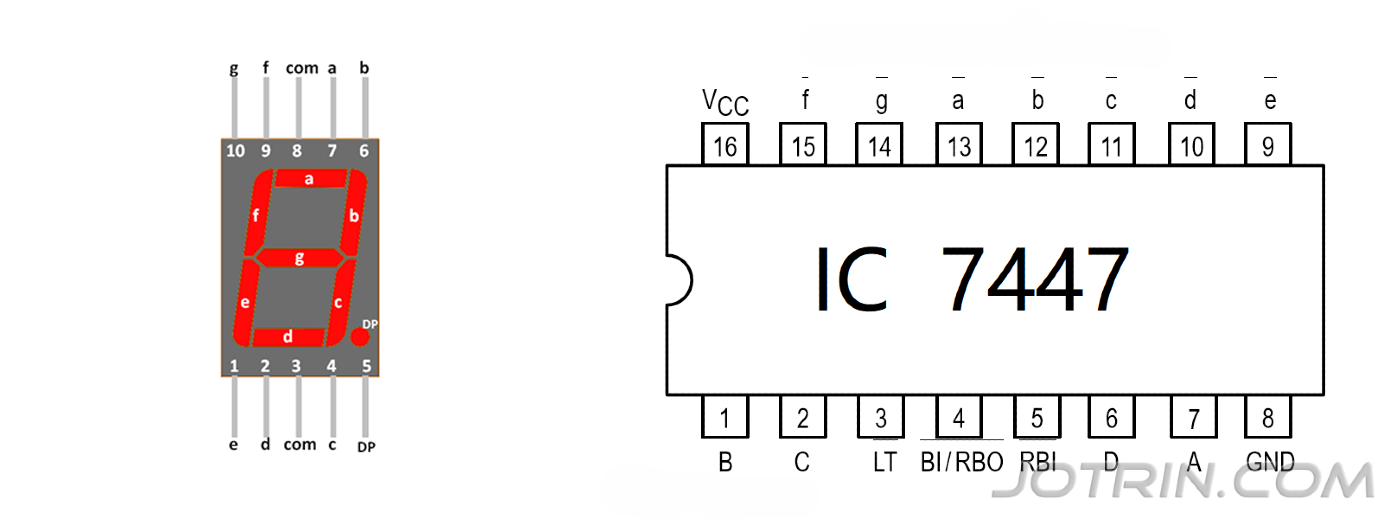
\includegraphics[width=\linewidth]{fig1.png}
    \caption{Caption}
    \label{fig:enter-label}
\end{figure}
\begin{table}[H]
    \centering
        \begin{tabular}{|c|c|}  % Adjust columns as needed
        \hline
        \textbf{Pin(Arduino)} & \textbf{Connected To} \\  % Header row
        \hline
        2,3,4,5 & A,B,C,D of 7447 IC \\  
        \hline
        6,7,8,9,10,11 & COM of all the 6 displays  \\ 
        \hline
        5V, GND & $V_{cc}$ and GND of 7447 IC  \\  
        \hline
    \end{tabular}

    \caption{Connections}
    \label{tab:my_label}
\end{table}
The seven-segment displays are  connected with each other so that all the inputs for all the displays are the same.
\section{Logic}
\begin{itemize}
    \item We can turn the displays on or off by controlling the digital pins (6-11).
    \item To change a digit at a specific position, we turn on only the corresponding display while keeping the others off. We then apply the updated digit value to the display.
    \item This switching happens very rapidly, so each display is turned off for only a very short time. Due to persistence of vision, our eyes perceive all displays as continuously lit.
\end{itemize}

\section{Multiplexing In Code}
Below is the implementation of the multiplexing logic in Embedded C:
\begin{lstlisting}[caption={Multiplexing Logic for 7-Segment Display}, label={lst:multiplexing}]
void displayTime() {
    uint8_t h1 = (hours >> 4) & 0x0F;  // Extract tens digit of hours
    uint8_t h2 = hours & 0x0F;         // Extract units digit of hours
    uint8_t m1 = (minutes >> 4) & 0x0F;
    uint8_t m2 = minutes & 0x0F;
    uint8_t s1 = (seconds >> 4) & 0x0F;
    uint8_t s2 = seconds & 0x0F;

    // Displaying each digit sequentially
    PORTD |= (1 << H1); displayDigit(h1); _delay_ms(5); PORTD &= ~(1 << H1);
    PORTD |= (1 << H2); displayDigit(h2); _delay_ms(5); PORTD &= ~(1 << H2);
    PORTB |= (1 << M1); displayDigit(m1); _delay_ms(5); PORTB &= ~(1 << M1);
    PORTB |= (1 << M2); displayDigit(m2); _delay_ms(5); PORTB &= ~(1 << M2);
    PORTB |= (1 << S1); displayDigit(s1); _delay_ms(5); PORTB &= ~(1 << S1);
    PORTB |= (1 << S2); displayDigit(s2); _delay_ms(5); PORTB &= ~(1 << S2);
}
\end{lstlisting}
\begin{itemize}
    \item \textbf{Digit Extraction}: Each digit for hours, minutes, seconds is stored in respective variables.
    \item \textbf{Activation of Displays}: The display is activated using PORTD(an 8bit register used to control the output of digital pins).
    \item \textbf{Delay}:5ms delay is introduced.
    \item \textbf{Deactivation}: The display is deactivated.
\end{itemize}

$$T_{display}=6 \times 5ms=30ms$$
On calling the function above the time is displayed for 30ms.\\
This function is repeatedly called inside the loop all the time is updated by Timer1 interrupts.



\section{Using Timer-1}
Below is the intialisation of Timer1
\begin{lstlisting}[caption={Multiplexing Logic for 7-Segment Display}, label={lst:multiplexing}]
void displayTime() {
    uint8_t h1 = (hours >> 4) & 0x0F;  // Extract tens digit of hours
    uint8_t h2 = hours & 0x0F;         // Extract units digit of hours
    uint8_t m1 = (minutes >> 4) & 0x0F;
    uint8_t m2 = minutes & 0x0F;
    uint8_t s1 = (seconds >> 4) & 0x0F;
    uint8_t s2 = seconds & 0x0F;

    // Displaying each digit sequentially
    PORTD |= (1 << H1); displayDigit(h1); _delay_ms(5); PORTD &= ~(1 << H1);
    PORTD |= (1 << H2); displayDigit(h2); _delay_ms(5); PORTD &= ~(1 << H2);
    PORTB |= (1 << M1); displayDigit(m1); _delay_ms(5); PORTB &= ~(1 << M1);
    PORTB |= (1 << M2); displayDigit(m2); _delay_ms(5); PORTB &= ~(1 << M2);
    PORTB |= (1 << S1); displayDigit(s1); _delay_ms(5); PORTB &= ~(1 << S1);
    PORTB |= (1 << S2); displayDigit(s2); _delay_ms(5); PORTB &= ~(1 << S2);
}
\end{lstlisting}
\begin{itemize}
    \item Timer1 generates an interrupt every second for updating the display.
    \item Ensures precise timekeeping.
\end{itemize}
\section{Conclusion}

\subsection{Advantages of Multiplexing}
\begin{itemize}
    \item \textbf{Reduces Hardware Requirements:} Using only one 7447 IC instead of separate decoder ICs for each display minimizes the number of components.
    \item \textbf{Lower Power Consumption:} At any given moment, only one display is actively drawing current, leading to lower overall power consumption.
    \item \textbf{Cost-Effective:} Since fewer components are required, the overall cost of the circuit is reduced.
    \item \textbf{Efficient Use of Microcontroller Pins:} Instead of dedicating multiple I/O pins to each display, we only use a few pins for selecting displays, making it ideal for resource-constrained microcontrollers.
\end{itemize}

\subsection{Disadvantages of Multiplexing}
\begin{itemize}
    \item \textbf{Processing Overhead:} The microcontroller continuously executes the multiplexing logic, consuming processing time that could otherwise be used for other tasks.
    \item \textbf{Perceived Brightness Reduction:} Since each display is turned on only for a fraction of the time, the brightness appears lower compared to direct driving methods.


\end{itemize}

\begin{figure}[H]
    \centering
    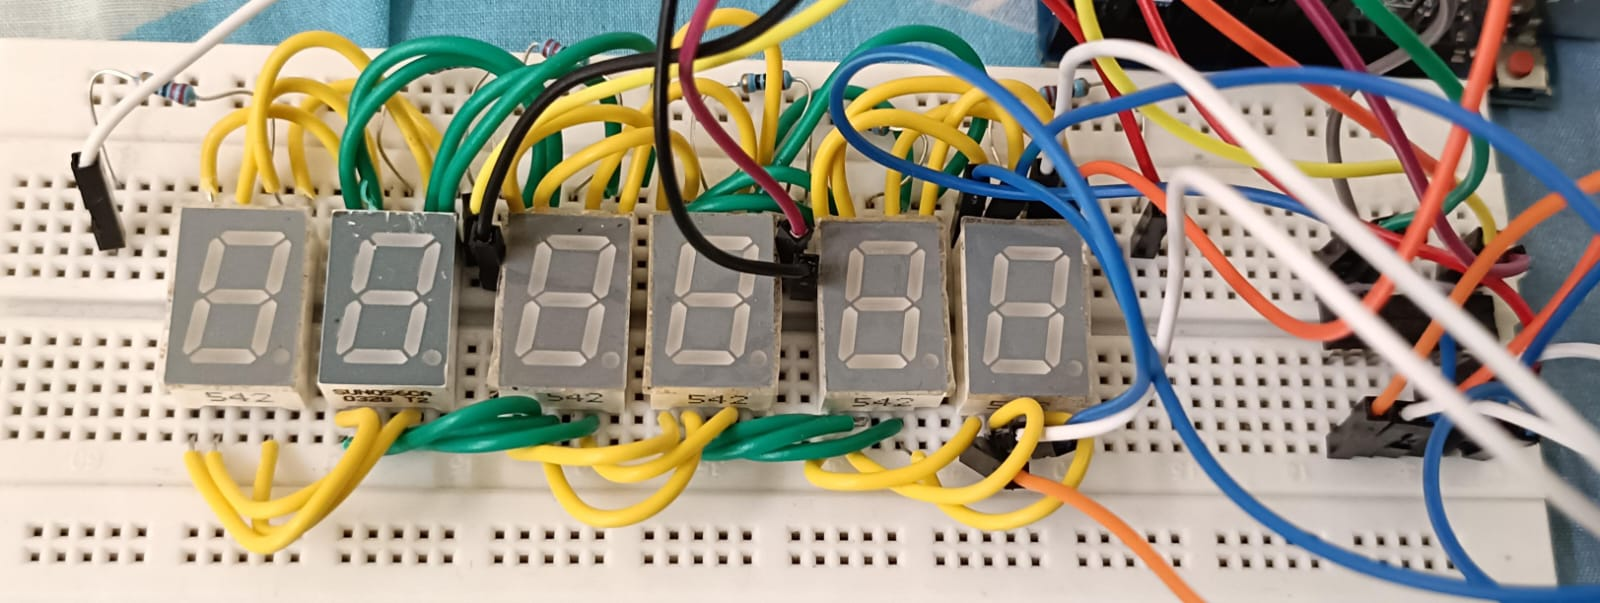
\includegraphics[width=\linewidth]{fig2.jpeg}
    \caption{Clock}
    \label{fig:enter-label}
\end{figure}




\end{document}

